\documentclass[11pt]{article}
\usepackage{geometry}                % See geometry.pdf to learn the layout options. There are lots.
\geometry{letterpaper}                   % ... or a4paper or a5paper or ... 
%\usepackage[parfill]{parskip}    % Activate to begin paragraphs with an empty line rather than an indent
\usepackage{graphicx}
%\usepackage{amssymb}
\usepackage{amsmath}
\usepackage{epstopdf}
\usepackage{natbib}
\usepackage{doi}
\usepackage{tikz}
\usetikzlibrary{arrows,decorations.markings}
\bibliographystyle{plainnat}
\DeclareGraphicsRule{.tif}{png}{.png}{`convert #1 `dirname #1`/`basename #1 .tif`.png}
\newcommand{\code}[1]{\mbox{\bf#1}}

\title{Regional MOM6}
\author{Kate Hedstrom \and Alistair Adcroft \and Robert Hallberg
\and Matt Harrison \and Maria Aristizabal \and Enrique Curchitser}
\date{}                                           % Activate to display a given date or no date

\begin{document}
\maketitle
\begin{abstract}
Adding and evaluating open boundary conditions (OBCs) in MOM6.
\end{abstract}
\section{Introduction}
\section{Methods}

The goal of this project is to add open boundary conditions (OBCs)
to MOM6 such that it can be used as a regional model. The open
boundaries can be placed anywhere on the model grid between q-points
on the Arakawa C grid, including but not limited to the domain
boundaries.  In fact, is is possible to create a staircase of open
boundary segments at an angle through the domain, such as seen in
Figure \ref{fdomain}. In order to support this feature, it is
necessary that nothing outside of the open boundary be used in the
model timestepping. If halo points were to be used, then both segments 2
and 3 in Figure \ref{fhalo} would be trying to set properties at
point A.

The following discussion will describe a boundary on the eastern
side of the domain, such as segment 4 in Figure \ref{fhalo}. See
Figure \ref{findices} for detailed placement on an Arakawa C grid.
Some options require a value for the boundary points; these will 
be denoted for example as $v_{\rm ext}$ for variable $v$. 

\begin{figure}
\begin{center}
\setlength{\unitlength}{10mm}
\begin{picture}(8.5,5.0)(0,0)
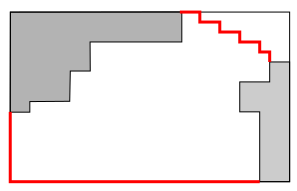
\includegraphics{pics/domain}
\end{picture}

\caption{An example of a domain with open boundary segments shown in red. Grey-shaded areas are land mask.}
\label{fdomain}
\end{center}
\end{figure}

\begin{figure}
\begin{center}
\setlength{\unitlength}{10mm}
%\begin{picture}
\begin{picture}(8,4.5)(0,0)

 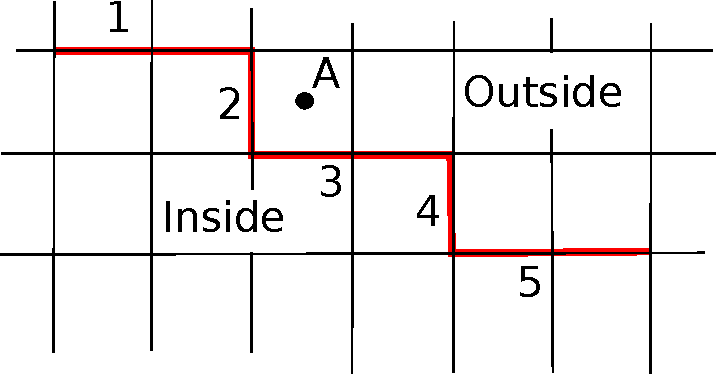
\includegraphics[width=8cm]{pics/halo}
\end{picture}
\caption{A portion of the grid with some numbered open boundary
segments. Point A is at a tracer point outside of OBC segments 2 and 3.}
\label{fhalo}
\end{center}
\end{figure}

\begin{figure}
\begin{center}
\setlength{\unitlength}{10mm}


\definecolor{cfd0000}{RGB}{253,0,0}


\begin{tikzpicture}[y=0.80pt, x=0.80pt, yscale=-1.000000, xscale=1.000000, inner sep=0pt, outer sep=0pt]
\begin{scope}[shift={(-163.5466,-431.83352)}]
  \path[draw=cfd0000,line join=miter,line cap=butt,miter limit=4.00,even odd
    rule,line width=3.200pt] (309.0437,474.0287) -- (308.5941,531.6145);
  \path[fill=black,miter limit=4.00,line width=3.200pt]
    (286.1362,503.0324)arc(0.000:89.505:5.311826 and
    4.903)arc(89.505:179.010:5.311826 and 4.903)arc(179.010:268.515:5.311826 and
    4.903)arc(268.515:358.019:5.311826 and 4.903);
  \path[draw=black,line join=miter,line cap=butt,even odd rule,line width=0.800pt]
    (164.7651,533.1417) -- (402.6996,532.0564);
  \path[draw=black,line join=miter,line cap=butt,even odd rule,line width=0.800pt]
    (163.5482,473.1356) -- (400.7699,472.3682);
  \path[draw=black,line join=miter,line cap=butt,even odd rule,line width=0.800pt]
    (250.5372,434.1369) -- (250.1654,569.4659);
  \path[draw=black,line join=miter,line cap=butt,even odd rule,line width=0.800pt]
    (369.4811,437.2064) -- (369.1094,572.5354);
  \path[draw=black,line join=miter,line cap=butt,even odd rule,line width=0.800pt]
    (308.8581,437.2064) -- (308.4863,572.5354);
  \path[draw=black,line join=miter,line cap=butt,even odd rule,line width=0.800pt]
    (189.9141,431.8347) -- (189.5424,567.1637);
  \path[fill=black,line join=miter,line cap=butt,line width=0.800pt]
    (304.3262,586.5253) node[above right] (text3379) {$i$};
  \path[fill=black,line join=miter,line cap=butt,line width=0.800pt]
    (176.4758,586.9905) node[above right] (text3383) {$i-2$};
  \path[fill=black,line join=miter,line cap=butt,line width=0.800pt]
    (236.3315,586.9905) node[above right] (text3387) {$i-1$};
  \path[fill=black,miter limit=4.00,line width=3.200pt]
    (226.2806,503.0324)arc(0.000:89.505:5.311826 and
    4.903)arc(89.505:179.010:5.311826 and 4.903)arc(179.010:268.515:5.311826 and
    4.903)arc(268.515:358.019:5.311826 and 4.903);
  \path[fill=black,line join=miter,line cap=butt,line width=0.800pt]
    (199.4973,553.2258) node[above right] (text3397) {$i-1.5$};
  \path[fill=black,line join=miter,line cap=butt,line width=0.800pt]
    (260.8877,554.7606) node[above right] (text3401) {$i-0.5$};
  \path[fill=black,line join=miter,line cap=butt,line width=0.800pt]
    (412.0616,477.2552) node[above right] (text3409) {$j$};
  \path[fill=black,line join=miter,line cap=butt,line width=0.800pt]
    (405.9225,535.5761) node[above right] (text3413) {$j-1$};
  \path[fill=black,line join=miter,line cap=butt,line width=0.800pt]
    (391.3423,506.4156) node[above right] (text3417) {$j-0.5$};
  \path[fill=black,line join=miter,line cap=butt,line width=0.800pt]
    (268.3021,517.2205) node[above right] (text3465) {$\eta$};
  \path[fill=black,line join=miter,line cap=butt,line width=0.800pt]
    (318.4652,515.7338) node[above right] (text3469) {$u$};
  \path[cm={{0.49092,-0.38205,0.38205,0.49092,(29.92447,456.97738)}},fill=black,miter
    limit=4.00,line width=0.800pt] (280.0000,382.3622) -- (277.0611,376.4073) --
    (270.4894,375.4524) -- (275.2447,370.8171) -- (274.1222,364.2720) --
    (280.0000,367.3622) -- (285.8779,364.2720) -- (284.7553,370.8171) --
    (289.5106,375.4524) -- (282.9389,376.4073) -- cycle;
  \path[cm={{0.49092,-0.38205,0.38205,0.49092,(29.92447,397.8891)}},fill=black,miter
    limit=4.00,line width=0.800pt] (280.0000,382.3622) -- (277.0611,376.4073) --
    (270.4894,375.4524) -- (275.2447,370.8171) -- (274.1222,364.2720) --
    (280.0000,367.3622) -- (285.8779,364.2720) -- (284.7553,370.8171) --
    (289.5106,375.4524) -- (282.9389,376.4073) -- cycle;
  \path[fill=black,line join=miter,line cap=butt,line width=0.800pt]
    (316.1631,466.1991) node[above right] (text3477) {$q$};
  \path[fill=black,line join=miter,line cap=butt,line width=0.800pt]
    (266.9305,463.8970) node[above right] (text3481) {$v$};
  \path[->,>=stealth,draw=black,line join=miter,line cap=butt,miter limit=4.00,even odd
    rule,line width=1.200pt] (300.0000,502.3622) -- (320.0000,502.3622);
  \path[->,>=stealth,draw=black,line join=miter,line cap=butt,miter limit=4.00,even odd
    rule,line width=1.200pt] (279.2807,482.4103) -- (279.3288,463.9932);
\end{scope}

\end{tikzpicture}



\caption{An eastern boundary segment at $i$ showing the staggered Arakawa C grid.}
\label{findices}
\end{center}
\end{figure}

\subsection{Barotropic}

\subsubsection{Specified}
For the barotropic mode, the only open boundary options are on the
velocity normal to a boundary segment. In the simplest case, one
knows both the barotropic velocity and the barotropic transport
through the OBC segments and can simply set them accordingly.
For a segment running north-south, one sets the $u$-velocity:
\begin{equation}
  \overline{u}_{i} = \overline{u}_{\rm ext}
\end{equation}
and the matching transport ($\overline{u} H dy$),
where $H$ is the total water depth and $dy$ is the meridional grid
spacing.

\subsubsection{Flather}

The original \citet{Flather76} algorithm is:
\begin{equation}
  \overline{u} = \overline{u}_{\rm ext} + \sqrt{\frac{g}{H}} \,
    (\eta - \eta_{\rm ext})
\end{equation}
The implementation used in MOM6 starts by finding a nondimensional
wave speed:
\begin{equation}
  C = \frac{dt}{dx} \sqrt{gH}
\end{equation}
then applying it to find an estimate of $\overline{u}$ and $\eta$ at the boundary.
If the boundary is at $i$ and we have an eastern boundary:
\begin{equation}
  u^{\star} = C \overline{u}^n_{i-1} + (1-C)\overline{u}^n_i
\end{equation}
\begin{equation}
  \eta^{\star} = \eta_{i-.5} + (0.5-C)(\eta_{i-.5} - \eta_{i-1.5})
\end{equation}
The new velocity becomes:
\begin{equation}
  \overline{u}^{n+1} = 0.5 \left( u^{\star} + \overline{u}_{\rm ext} +
    \sqrt{\frac{g}{H}} (\eta^{\star} - \eta_{\rm ext}) \right)
\end{equation}
The velocity used in the transport equation has some time filtering applied:
\begin{equation}
  \overline{u}_{\rm trans} = (1 - \beta)\overline{u}^n + \beta \overline{u}^{n+1}
\end{equation}
with $\beta > 0.05$ often set to 0.2.
[I don't know why the transport is filtered and not ubt directly.]

\subsection{Baroclinic normal velocity}
\subsubsection{Specified}
Much like the barotropic option, one simply sets the normal flow
and the normal transport:
\begin{equation}
  u_{i} = u_{\rm ext}
\end{equation}
and the matching transport ($u h dy$),
where $h$ is the layer depth and $dy$ is the meridional grid
spacing.

\subsubsection{Gradient}
Setting the gradient to zero at the boundary requires no
external values:
\begin{equation}
  u_{i} = u_{i-1}
\end{equation}

\subsubsection{Radiation}
In realistic domains, open boundary conditions can be extremely
difficult to get right. There are situations in which incoming flow and
outgoing flow happen along the same boundary or even at different
depths at the same horizontal location. \citet{Orlanski76}
proposed a radiation scheme in which a local normal phase velocity is
computed and used to radiate things out (if it is indeed going out).
This works well for a wave propagating normal to the boundary, but
has problems when waves approach the boundary at an angle.
\citet{Raymond84} have modified the scheme to account for
propagation in all three directions. In ROMS, only the two horizontal
directions are accounted for (with the recommended \code{RADIATION\_2D}
option):
\begin{equation}
   \frac{\partial \phi}{\partial t} = - \left( \phi_\xi \frac{\partial
   \phi}{\partial \xi} + \phi_\eta \frac{\partial \phi}{\partial \eta}) \right)
\label{eqrk}
\end{equation}
where
\begin{align}
  \phi_\xi & = \frac{F \frac{\partial \phi}{\partial \xi}}{
  \left( \frac{\partial \phi}{\partial \xi} \right)^2 +
  \left( \frac{\partial \phi}{\partial \eta} \right)^2 } \\ 
  \phi_\eta & = \frac{F \frac{\partial \phi}{\partial \eta}}{
  \left( \frac{\partial \phi}{\partial \xi} \right)^2 +
  \left( \frac{\partial \phi}{\partial \eta} \right)^2 } \\ 
   F & = - \frac{\partial \phi}{\partial t}
\end{align}
These terms are evaluated at the closest interior point in a manner
consistent with the time stepping scheme used. The phase velocities are
limited so that the local Courant-Friedrichs-Lewy (CFL) condition
is satisfied. They are then
applied to the boundary point using equation (\ref{eqrk}), again using
a consistent time stepping scheme. Raymond and Kuo give the form used
for centered differencing and a leapfrog time step while ROMS uses
one-sided differences.

The radiation approach is appropriate for waves leaving the domain. A
check is made to see which way the phase velocity is headed. If it
is entering the domain, a zero gradient condition is applied unless
an additional nudging option is also specified as described below.

\subsubsection{Mixed radiation-nudging boundary condition}
As described in \citep{Marchesiello2001}, ROMS has an option for providing
radiation conditions on outflow and nudging to a known exterior
value on inflow. This is implemented as a variation on the radiation
condition, requiring two timescales: the inflow nudging timescale and the
outflow nudging timescale. These timescales are provided in the input to
ROMS (\S\ref{ASCII_in}).

\subsection{Tangential velocity}
\subsubsection{Vorticity}
\subsubsection{Strain}
\subsection{Tracers}
\section{Test problems}
\subsection{Barotropic Kelvin wave}
\subsection{Tracers}
\section{A realistic problem}
\section{Conclusions}
\section{Discussion}


\bibliography{ocean}
\end{document}  
